\section{Referenzmodellierung}\label{theorie:referenzmodellierung}
Gemäß des konstruktionsprozessorientierten Referenzmodellbegriffs von vom Brocke ist ein Referenzmodell als solches zu erkennen, wenn der Gegenstand und/oder\footnote{Die Verwendung von \enquote{und/oder} wurde hier gewählt, da der Autor der Quelle das \enquote{oder} aus der boolschen Algebra gewählt hat um explizit beide Fälle einzuschliessen.} der Inhalt des Referenzmodells bei der Konstruktion des Gegenstandes und/oder des Inhaltes eines zu konstruierenden Anwendungsmodells wiederverwendet werden kann.\footcite[Vgl.][34]{vomBrocke.2003} Dabei hat ein Referenzmodell einen Empfehlungscharakter und stellt eine \enquote{best practice} dar.\footcite[Vgl.][31]{vomBrocke.2003} 


\Todo{Grundsätze ordnungsgemäßer Modellierung - siehe auch 148 vomBrocke.2003}

\begin{figure}[H]
\centering
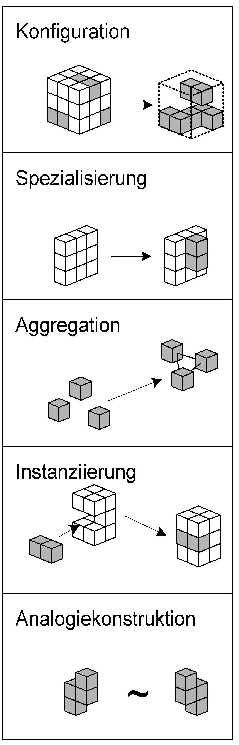
\includegraphics[height=0.45\textheight]{graphics/anwendung-referenzmodelle.pdf}
\caption[Konstruktionstechniken der Referenzmodellierung]{Konstruktionstechniken der Referenzmodellierung.\footnotemark}
\label{abb:KonstruktionstechnikenRefMod}
\end{figure}
\footnotetext{Mit Änderungen entnommen aus: \cite[][262]{vomBrocke.2003}}
\Todo{Einsatzszenarien darstellen (Konfiguration, ...)}

Ein Referenzmodell kann nach vom Brocke nicht objektiv allgemeingültig sein und auch keinen objektiven Empfehlungscharakter haben, sondern muss subjektiv beurteilt werden.\footcite[Vgl. auch im Folgenden][31~f.]{vomBrocke.2003}  Dabei ist zumindest von den Interessensgruppen der Konstruierenden und der Nutzenden auszugehen, welche das Referenzmodell subjektiv unterschiedlich nach Allgemeingültigkeit und Empfehlungscharakter bewerten. Je nachdem welche Beurteilung höher gewichtet wird und früher einfließt, kann also entweder von der Situation ausgegangen werden, dass das Referenzmodell vom Konstruierenden zu einem solchen erklärt wird oder ein Modell, ob vom Konstruierenden beabsichtigt oder nicht, von den Nutzenden zu einem solchen erhoben wird.

% Um einen möglichst hohen Nutzen stiften zu können, müssen die organisatorischen Rahmenbedingungen, in welchen ein Referenzmodell eingesetzt werden soll analysiert werden.\footcite[Vgl.][]{vomBrocke.2004}

Im Rahmen dieser Arbeit entwickelte Modelle ordnen sich der Infrastrukturarchitektur unter. Die Infrastruktur umfasst nach Definition von Lichtenegger u.a. die Beschreibung der Software-, Hardware und Netzwerkinfrastruktur, die zum Betrieb von Applikationen erforderlich ist. \Todo{Bessere Definition} Auch die hier zu entwickelnden Referenzarchitekturen für Datenverarbeitung zählen dabei nach der in diesem Kapitel erläuterten Defintion von vom Brocke als Referenzmodelle, da sie explizit zur Wiederverwendung konstruiert wurden.

Zur Darstellung der verwendeten Produkte in den Referenzmodellen und des Datenflusses soll die erste Stufe der Bausteinsicht des Architekturstandards arc42 verwendet werden. Das Konzept jener Bausteinsicht, also wie sie zu gestalten ist, findet sich in \autoref{abb:BausteinsichtStufe1}. In derr finalen Umsetzung werden die offiziellen \ac{AWS} Icons die entsprechenden Services darstellen, die verwendet werden.

\begin{figure}[H]
\centering
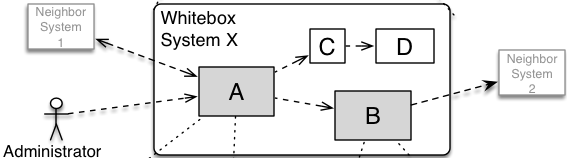
\includegraphics[width=\textwidth]{graphics/erste-Stufe-Bausteinsicht.png}
\caption[Stufe 1 der Bausteinsicht in arc42]{Stufe 1 der Bausteinsicht in arc42.\footnotemark}
\label{abb:BausteinsichtStufe1}
\end{figure}
\footnotetext{Mit Änderungen entnommen aus: \cite{Starke.o.J.}}



% Überleitung => generelle Referenzmodelle 
% => Empfehlungscharakter 
% => Anwendung Architektur 
% => Unterlegung Arc42 als Modellierungssprache

